\documentclass{article}

\def\npart {IA}
\def\nterm {Lent}
\def\nyear {2024}
\def\nlecturer {Prof. D.\ Tong}
\def\ncourse {Vector Calculus}

\setcounter{tocdepth}{2}

\usepackage{alltt}
\usepackage{amsmath, amsfonts, amssymb, amsthm}
\usepackage{booktabs}
\usepackage{caption}
\usepackage{enumitem}
\usepackage{fancyhdr}
\usepackage{graphicx}
\usepackage{mathdots}
\usepackage{mathtools}
\usepackage{microtype}
\usepackage{multirow}
\usepackage{pdflscape}
\usepackage{pgfplots}
\usepackage{siunitx}
\usepackage{textcomp}
\usepackage{slashed}
\usepackage{tabularx}
\usepackage{tikz}
\usepackage{tkz-euclide}
\usepackage[normalem]{ulem}
\usepackage[all]{xy}

\pgfplotsset{compat=1.18}
\pagestyle{fancyplain}

\lhead{\emph{\nouppercase{\leftmark}}}
\rhead{
  \ifnum\thepage=1
  \else
    \npart\ \vline\ \ncourse
  \fi}

\def\nauthor{Marcus Ng}
\author{Based on lectures by \nlecturer \\\small Notes taken by \nauthor}
\date{\nterm\ \nyear}
\title{Part \npart\ --- \ncourse}

\newcommand*{\Cdot}{{\raisebox{-0.25ex}{\scalebox{1.5}{$\cdot$}}}}
\setlist[enumerate,1]{label={(\roman*)}}

\newcommand {\pd}[2][ ]{
  \ifx #1 { }
    \frac{\partial}{\partial #2}
  \else
    \frac{\partial^{#1}}{\partial #2^{#1}}
  \fi
}

% Theorems
\theoremstyle{definition}
\newtheorem*{aim}{Aim}
\newtheorem*{axiom}{Axiom}
\newtheorem*{claim}{Claim}
\newtheorem*{cor}{Corollary}
\newtheorem*{conjecture}{Conjecture}
\newtheorem*{defi}{Definition}
\newtheorem*{eg}{Example}
\newtheorem*{ex}{Exercise}
\newtheorem*{fact}{Fact}
\newtheorem*{law}{Law}
\newtheorem*{lemma}{Lemma}
\newtheorem*{notation}{Notation}
\newtheorem*{prop}{Proposition}
\newtheorem*{question}{Question}
\newtheorem*{problem}{Problem}
\newtheorem*{rrule}{Rule}
\newtheorem*{thm}{Theorem}
\newtheorem*{assumption}{Assumption}
\newtheorem*{assert}{Assertion}

\newtheorem*{remark}{Remark}
\newtheorem*{warning}{Warning}
\newtheorem*{exercise}{Exercise}

\newtheorem{nthm}{Theorem}[section]
\newtheorem{nlemma}[nthm]{Lemma}
\newtheorem{nprop}[nthm]{Proposition}
\newtheorem{ncor}[nthm]{Corollary}

\SetEnumitemKey{cases}{
  label=\underline{Case~\arabic*:},
  ref={\arabic*},
  align=left,
  leftmargin=\parindent
}

% \renewcommand{\labelitemi}{--}
% \renewcommand{\labelitemii}{$\circ$}
% \renewcommand{\labelenumi}{(\roman{*})}

\let\stdsection\section
\renewcommand\section{\newpage\stdsection}

% Strike through
\def\st{\bgroup \ULdepth=-.55ex \ULset}


%%%%%%%%%%%%%%%%%%%%%%%%%
%%%%% Maths Symbols %%%%%
%%%%%%%%%%%%%%%%%%%%%%%%%

% Logical symbols
\newcommand{\contradiction}{
  
\begin{tikzpicture}[rotate=45,x=0.5ex,y=0.5ex]
  \draw[line width=.1ex] (0,2) -- (3,2) (0,1) -- (3,1) (1,3) -- (1,0) (2,3) -- (2,0);
  \end{tikzpicture}
}


\let\U\relax
\let\C\relax
\let\G\relax

% Matrix groups
% \newcommand{\GL}{\mathrm{GL}}
% \newcommand{\Or}{\mathrm{O}}
% \newcommand{\PGL}{\mathrm{PGL}}
% \newcommand{\PSL}{\mathrm{PSL}}
% \newcommand{\PSO}{\mathrm{PSO}}
% \newcommand{\PSU}{\mathrm{PSU}}
% \newcommand{\SL}{\mathrm{SL}}
% \newcommand{\SO}{\mathrm{SO}}
% \newcommand{\Spin}{\mathrm{Spin}}
% \newcommand{\Sp}{\mathrm{Sp}}
% \newcommand{\SU}{\mathrm{SU}}
\newcommand{\U}{\mathrm{U}}
% \newcommand{\Mat}{\mathrm{Mat}}

% Matrix algebras
% \newcommand{\gl}{\mathfrak{gl}}
% \newcommand{\ort}{\mathfrak{o}}
% \newcommand{\so}{\mathfrak{so}}
% \newcommand{\su}{\mathfrak{su}}
% \newcommand{\uu}{\mathfrak{u}}
% \renewcommand{\sl}{\mathfrak{sl}}

% Special sets
\newcommand{\C}{\mathbb{C}}
\newcommand{\CP}{\mathbb{CP}}
\newcommand{\GG}{\mathbb{G}}
\newcommand{\N}{\mathbb{N}}
\newcommand{\Q}{\mathbb{Q}}
\newcommand{\R}{\mathbb{R}}
\newcommand{\RP}{\mathbb{RP}}
\newcommand{\T}{\mathbb{T}}
\newcommand{\Z}{\mathbb{Z}}
\renewcommand{\H}{\mathbb{H}}

% Brackets
\newcommand{\abs}[1]{\left\lvert #1\right\rvert}
\newcommand{\bket}[1]{\left\lvert #1\right\rangle}
\newcommand{\brak}[1]{\left\langle #1 \right\rvert}
\newcommand{\braket}[2]{\left\langle #1\middle\vert #2 \right\rangle}
\newcommand{\bra}{\langle}
\newcommand{\ket}{\rangle}
\newcommand{\norm}[1]{\left\lVert #1\right\rVert}
\newcommand{\normalorder}[1]{\mathop{:}\nolimits\!#1\!\mathop{:}\nolimits}
\newcommand{\tv}[1]{|#1|}
\renewcommand{\vec}[1]{\boldsymbol{\mathbf{#1}}}

% not-math
% \newcommand{\bolds}[1]{{\bfseries #1}}
% \newcommand{\cat}[1]{\mathsf{#1}}
% \newcommand{\ph}{\,\cdot\,}
% \newcommand{\term}[1]{\emph{#1}\index{#1}}
% \newcommand{\phantomeq}{\hphantom{{}={}}}

% Probability
% \DeclareMathOperator{\Bernoulli}{Bernoulli}
% \DeclareMathOperator{\betaD}{beta}
% \DeclareMathOperator{\bias}{bias}
% \DeclareMathOperator{\binomial}{binomial}
% \DeclareMathOperator{\corr}{corr}
% \DeclareMathOperator{\cov}{cov}
% \DeclareMathOperator{\gammaD}{gamma}
% \DeclareMathOperator{\mse}{mse}
% \DeclareMathOperator{\multinomial}{multinomial}
% \DeclareMathOperator{\Poisson}{Poisson}
% \DeclareMathOperator{\var}{var}
% \newcommand{\E}{\mathbb{E}}
% \newcommand{\Prob}{\mathbb{P}}

% Algebra
% \DeclareMathOperator{\adj}{adj}
% \DeclareMathOperator{\Ann}{Ann}
% \DeclareMathOperator{\Aut}{Aut}
% \DeclareMathOperator{\Char}{char}
% \DeclareMathOperator{\disc}{disc}
% \DeclareMathOperator{\dom}{dom}
% \DeclareMathOperator{\fix}{fix}
% \DeclareMathOperator{\Hom}{Hom}
% \DeclareMathOperator{\id}{id}
% \DeclareMathOperator{\image}{image}
% \DeclareMathOperator{\im}{im}
% \DeclareMathOperator{\re}{re}
% \DeclareMathOperator{\tr}{tr}
% \DeclareMathOperator{\Tr}{Tr}
% \newcommand{\Bilin}{\mathrm{Bilin}}
% \newcommand{\Frob}{\mathrm{Frob}}

% Others
% \newcommand\ad{\mathrm{ad}}
% \newcommand\Art{\mathrm{Art}}
% \newcommand{\B}{\mathcal{B}}
% \newcommand{\cU}{\mathcal{U}}
% \newcommand{\Der}{\mathrm{Der}}
% \newcommand{\D}{\mathrm{D}}
% \newcommand{\dR}{\mathrm{dR}}
% \newcommand{\exterior}{\mathchoice{{\textstyle\bigwedge}}{{\bigwedge}}{{\textstyle\wedge}}{{\scriptstyle\wedge}}}
% \newcommand{\F}{\mathbb{F}}
% \newcommand{\G}{\mathcal{G}}
% \newcommand{\Gr}{\mathrm{Gr}}
% \newcommand{\haut}{\mathrm{ht}}
% \newcommand{\Hol}{\mathrm{Hol}}
% \newcommand{\hol}{\mathfrak{hol}}
% \newcommand{\Id}{\mathrm{Id}}
% \newcommand{\lie}[1]{\mathfrak{#1}}
% \newcommand{\op}{\mathrm{op}}
% \newcommand{\Oc}{\mathcal{O}}
% \newcommand{\pr}{\mathrm{pr}}
% \newcommand{\Ps}{\mathcal{P}}
% \newcommand{\pt}{\mathrm{pt}}
% \newcommand{\qeq}{\mathrel{``{=}"}}
% \newcommand{\Rs}{\mathcal{R}}
% \newcommand{\Vect}{\mathrm{Vect}}
% \newcommand{\wsto}{\stackrel{\mathrm{w}^*}{\to}}
% \newcommand{\wt}{\mathrm{wt}}
% \newcommand{\wto}{\stackrel{\mathrm{w}}{\to}}
% \renewcommand{\d}{\mathrm{d}}
% \renewcommand{\P}{\mathbb{P}}
%\renewcommand{\F}{\mathcal{F}}

\let\Im\relax
\let\Re\relax

% \DeclareMathOperator{\area}{area}
% \DeclareMathOperator{\card}{card}
% \DeclareMathOperator{\ccl}{ccl}
% \DeclareMathOperator{\ch}{ch}
% \DeclareMathOperator{\cl}{cl}
% \DeclareMathOperator{\cls}{\overline{\mathrm{span}}}
% \DeclareMathOperator{\coker}{coker}
% \DeclareMathOperator{\conv}{conv}
% \DeclareMathOperator{\cosec}{cosec}
% \DeclareMathOperator{\cosech}{cosech}
% \DeclareMathOperator{\covol}{covol}
% \DeclareMathOperator{\diag}{diag}
% \DeclareMathOperator{\diam}{diam}
% \DeclareMathOperator{\Diff}{Diff}
% \DeclareMathOperator{\End}{End}
% \DeclareMathOperator{\energy}{energy}
% \DeclareMathOperator{\erfc}{erfc}
% \DeclareMathOperator{\erf}{erf}
% \DeclareMathOperator*{\esssup}{ess\,sup}
% \DeclareMathOperator{\ev}{ev}
% \DeclareMathOperator{\Ext}{Ext}
% \DeclareMathOperator{\fst}{fst}
% \DeclareMathOperator{\Fit}{Fit}
% \DeclareMathOperator{\Frac}{Frac}
% \DeclareMathOperator{\Gal}{Gal}
% \DeclareMathOperator{\gr}{gr}
% \DeclareMathOperator{\hcf}{hcf}
\DeclareMathOperator{\Im}{Im}
% \DeclareMathOperator{\Ind}{Ind}
% \DeclareMathOperator{\Int}{Int}
% \DeclareMathOperator{\Isom}{Isom}
% \DeclareMathOperator{\lcm}{lcm}
% \DeclareMathOperator{\length}{length}
% \DeclareMathOperator{\Lie}{Lie}
% \DeclareMathOperator{\like}{like}
% \DeclareMathOperator{\Lk}{Lk}
% \DeclareMathOperator{\Maps}{Maps}
% \DeclareMathOperator{\orb}{orb}
% \DeclareMathOperator{\ord}{ord}
% \DeclareMathOperator{\otp}{otp}
% \DeclareMathOperator{\poly}{poly}
% \DeclareMathOperator{\rank}{rank}
% \DeclareMathOperator{\rel}{rel}
% \DeclareMathOperator{\Rad}{Rad}
\DeclareMathOperator{\Re}{Re}
% \DeclareMathOperator*{\res}{res}
% \DeclareMathOperator{\Res}{Res}
% \DeclareMathOperator{\Ric}{Ric}
% \DeclareMathOperator{\rk}{rk}
% \DeclareMathOperator{\Rees}{Rees}
% \DeclareMathOperator{\Root}{Root}
% \DeclareMathOperator{\sech}{sech}
% \DeclareMathOperator{\sgn}{sgn}
% \DeclareMathOperator{\snd}{snd}
% \DeclareMathOperator{\Spec}{Spec}
% \DeclareMathOperator{\spn}{span}
% \DeclareMathOperator{\stab}{stab}
% \DeclareMathOperator{\St}{St}
% \DeclareMathOperator{\supp}{supp}
% \DeclareMathOperator{\Syl}{Syl}
% \DeclareMathOperator{\Sym}{Sym}
% \DeclareMathOperator{\vol}{vol}
\numberwithin{equation}{section}

\begin{document}
\maketitle{
    \small 
    \noindent\textbf{Curves in $\R^3$}\\
    Parameterised curves and arc length, tangents and normals to curves in $\R^3$; curvature and torsion.\hspace*{\fill}[1]
    
    \vspace{10pt}
    \noindent\textbf{Integration in $\R^2$ and $\R^3$}\\
    Line integrals. Surface and volume integrals: definitions, examples using Cartesian, cylindrical and spherical coordinates; change of variables.\hspace*{\fill}[4]

    \vspace{10pt}
    \noindent\textbf{Vector operations}\\
    Directional derivatives. The gradient of a real-valued function: definition; intterpretation as normal to level surfaces;
    examples including the use of cylindrical, spherical *and general curvilinear* coordinates
    
    \vspace{5pt}
    \noindent Divergence, curl and $\nabla^2$ in Cartesian coordinates, examples; 
    formulae for these operators (statement only) in cylindrical, spherical *and general curvilinear* coordinates. 
    Solenoidal fields, irrotational fields and conservative fields; scalar potentials. Vector derivative identities \hspace*{\fill}[5]
    
    \vspace{10pt}
    \noindent\textbf{Integration theorems}\\
    Divergence theorem, Green's theorem, Stoke's theorem, Green's second theorem: statement;
    informal proofs; examples; applications to fluid dynamics, and to electromagnetism including statement of Maxwell's equations. \hspace*{\fill}[5]

    \vspace{10pt}
    \noindent\textbf{Laplace's equation}\\
    Laplace's equation in $\R^2$ and $\R^3$: uniqueness theorem and maximum principle. 
    Solution of Poisson's equation by Gauss's method (for spherical and cylindrical symmetry) and as an integral. \hspace*{\fill}[4]

    \vspace{10pt}
    \noindent\textbf{Cartesian tensors in $\R^3$}\\
    Tensor transformation laws, addition, multiplication, contraction, with emphasis on tensors of second rank.
    Isotropic second and third rank tensors. Symmetric and antisymmetric tensors. Revision of principal axes and diagonalisation.
    Quotient theorem. Examples indlucing inertia and conductivity.\hspace*{\fill}[5]
}
\tableofcontents

%%%%%%%%%%%%%%%%%%%%%%
% Lecture 1: 18/01/2024
%%%%%%%%%%%%%%%%%%%%%%

\section*{Introduction}
We will learn to differentiate and integrate functions (or maps) of the form
\[f : \R^m \rightarrow \R^n\]
and element of $\R^m$ or $\R^n$ is a vector, so this subject is called ``vector calculus''.

\begin{eg}[Maps]\leavevmode
    \begin{enumerate}
        \item A function $f: \R \rightarrow \R^n$ defines a \emph{curve} in $\R^n$.
        In physics, we think of the domain as time, and the codomain as space, (usually with $n = 3$), and we write this as
        \[ f: t \mapsto \vec x(t)\] 
        with $\vec x(t) \in \R^n$. Generalising, a map $f: \R^2 \rightarrow \R^n$ defines a \emph{surface} in $\R^n$, and so on.

        \item In other applications, the domain $\R^m$ might be viewed as physical space. 
        For example, in physics a \emph{scalar field} is a map
        \[f: \R^3 \rightarrow \R\]
        For example, temperature $T(\vec x)$ is an example of a scalar field, as is the Higgs boson field.
        
        \item A \emph{vector field} is a map $f: \R^3 \rightarrow R^n$.
        For example, the electric field $\vec E(x)$ and the magnetic field $\vec B(x)$ are vector fields. 
    \end{enumerate}
\end{eg}

\section{Curves}
We consider maps of the form $f: \R \rightarrow \R^n$. 
Assign a coordiante $t$ to $\R$ and use cartesian coordiantes on $\R^n$
\[ \vec x = (\vec x^1, \cdots \vec x^n) = x^i \vec e_i \tag{summation notation over $i$}\]

\begin{notation}
In this course, the lecture will use super-scripts i.e. $\vec x^i$ to denote the the $i^{th}$ component of the vector $\vec x$.
He mentions something about this being the right way to do things, but that this will only bear fruit in future courses.
\end{notation}

With $\vec e_i$ the orthonormal basis of $\R^n$ such that
\[\vec e_i \cdot \vec e_j = \delta_{ij}\]
In expanded form,
\begin{align*}
    \vec e_1 &= (1, 0, \cdots, 0) \\
    \vec e_2 &= (0, 1, \cdots, 0) \\
    \vdots & \\
    \vec e_n &= (0, 0, \cdots, 1)
\end{align*}

For $\R^3$ we also use the notation
\[\{\vec e_i\} = \{\uvec x, \uvec y, \uvec z\}\]
The image of the function is a \emph{parameterised curve}, with $t$ the parameter. We call the curve $C$.

\begin{eg}\leavevmode
\begin{enumerate}
    \item Consider the map $\R \rightarrow \R^3$ given by 
    \[\vec x(t) = (at, bt^2, 0)\]
    The curve $C$ is the parabola $a^2y = b^2x$ lying in the plane $z = 0$.
    \begin{center}
        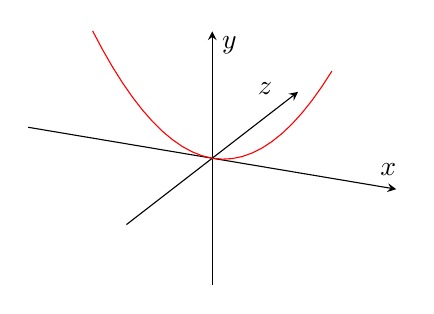
\begin{tikzpicture}
            \begin{axis}[
                axis lines=center,
                xlabel = $x$,
                ylabel = $z$,
                zlabel = $y$,
                xtick=\empty,
                ytick=\empty,
                ztick=\empty,
                xmin=-2,
                xmax=2,
                ymin=-2,
                ymax=2,
                zmin=-2,
                zmax=2
            ]
            \addplot3[
                color=red,
                variable=\t,
                domain=-1.3:1.3,
                samples y=0
            ]
            (\t, 0, \t^2);
            \end{axis}
        \end{tikzpicture}
    \end{center}

    \item Consider $\vec x (t) = (\cos t, \sin t, t)$. The curve $C$ is a helix
    \begin{center}
        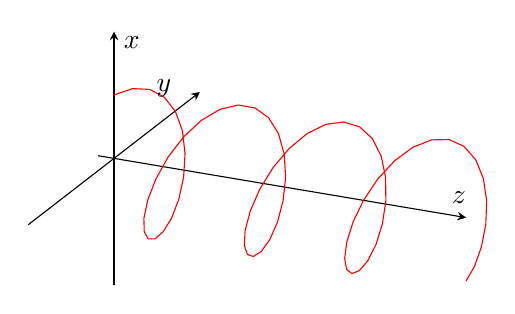
\begin{tikzpicture}
            \begin{axis}[
                axis lines=center,
                xlabel = $z$,
                ylabel = $y$,
                zlabel = $x$,
                xtick=\empty,
                ytick=\empty,
                ztick=\empty,
                xmin=-1,
                xmax=7*pi,
                ymin=-2,
                ymax=2,
                zmin=-2,
                zmax=2
            ]
            \addplot3[
                color=red,
                variable=\t,
                domain=0:7*pi,
                samples=70,
                samples y=0
            ]
            (\t, {sin(\t r)}, {cos(\t r)});
            \end{axis}
        \end{tikzpicture}
    \end{center}
    Note that the choice of paramterisation is not unique!
    For example, consider $\vec x(t) = (\cos \lambda t, \sin \lambda t, \lambda t)$ gives the same helix $\forall \lambda \neq 0$.
    Sometimes, the choice of paramterisation matters. i.e, if $t$ is the time and $\vec x(t)$ is position, then the velocity $\dvec x \propto \lambda$
\end{enumerate}
\end{eg}

\subsection{Differentiating the Curve}
A vector function $\vec x(t)$ is said to be differentiable at $t$ if as $\delta t \rightarrow 0$ we have
\[ \vec x(t + \delta t) - \vec x(t) = \dvec x(t)\delta t + O(\delta t^2)\]
Note that we use this to define $\dvec x(t)$ at the point $t$.
If $\dvec x(t)$ exists everywhere, then the curve is said to be \emph{smooth}.

\begin{remark}
    \begin{enumerate}
        \item ``Big O'' notation $O(\delta t^2)$ means terms proportional to $\delta t^2$
        \item ``Little O'' notation $\underline{o}(\delta t^2)$ means strictly smaller than $\delta t^2$
        \item In physics, dot is usually used to denote differentiation with respect to time ($\dvec x(t)$).
        The prime is used for spatial differentiation ($f'(x)$). In maths, these are used interchangably.
    \end{enumerate}
\end{remark}

\begin{notation}
    We write
    \[
        \delta \vec x(t) = \vec x(t + \delta t) - \vec x(t)   
    \]
    The derivative is then
    \[ \dvec x(t) \equiv \diff {\vec x}{t} := \lim_{\delta t \rightarrow 0} \frac{\delta \vec x}{\delta t}\]
    We also sometimes write
    \[ \diffd \vec x := \dvec x \diffd t\]
\end{notation}

\end{document}